\documentclass{article}

\usepackage{graphicx}
\usepackage{amsmath}
\usepackage{color}
\usepackage{subfigure}
\usepackage{enumerate}

\oddsidemargin=-.5cm
\evensidemargin=-.5cm
\textwidth=17cm
\topmargin=-2cm
\textheight=23cm
\newcommand{\pd}{{\vphantom\dagger}}
\newcommand{\de}{\bar{\delta}}
\newcommand{\Li}{\bar{L}}

\title{Scaling of entanglement entropy in the RVB wavefunction}
\begin{document}

\maketitle

\section{Simulations}
Using Monte Carlo simulations in the valence bond basis, we study the SU(N) RVB wavefunction.
The RVB wavefunction is an equal-amplitude superposition of all nearest-neighbor valence-bond states, $| \Psi \rangle = \sum_{\langle i j \rangle} | \phi \rangle_{ij}$, where
%
\begin{equation}
	\displaystyle
	\label{eq:wf}
	| \phi \rangle_{ij} = \frac{1}{2S + 1} \sum_{m = -S}^{S} \, (-1)^{m-S} \, | m \rangle_i \otimes \, | -m \rangle_j,
\end{equation}
%
in the $S^z$ basis $(2S+1 \equiv N)$.
Here, $i, j$ are nearest neighbor sites on the square lattice.
Because the wavefunction is inversely proportional to $N \equiv 2S+1$, as $N \to \infty$, the RVB wavefunction approaches the limit of classical dimers, where the states $\phi$ are orthogonal.
The RVB Monte Carlo sampling algorithm does a random walk through the possible states by creating a defect at some spatial point and propagating it through the system (thereby rearranging the nearest-neighbor bonds) until the defect reaches the initial point and its path forms a closed loop.

We give the estimators for the correlation functions.
Details can be found in Beach's paper.
We wish to compute the dimer-dimer correlation function
%
\begin{equation}
	\langle D_i(r) \,D_j(r') \rangle \sim \langle (S_r \cdot S_{r+\hat{e}_i} ) (S_{r'} \cdot S_{r'+\hat{e}_j}) \rangle
			 - \langle S_r \cdot S_{r+\hat{e}_i} \rangle  \langle S_{r'} \cdot S_{r'+\hat{e}_j}\rangle.
\end{equation}
%
The spin-spin correlations:
%
\begin{equation}
	\langle S_r \cdot S_{r+\hat{e}_i} \rangle = \epsilon_{r,r'} \, S ( S+1),
\end{equation}
%
where $\epsilon_{r,r'} = 1$ if $r,r'$ are on the same sublattice and $-1$ otherwise.
%
In the simulations, we compute only parallel dimer-dimer correlations, i.e. $D_y(r) \, D_y(r+ n \hat{e}_x)$, with $n = 0, 1, ..$.
The estimators are
%
\begin{equation}
\displaystyle
D_y(r) \, D_y(r') = 
	\left\{ \begin{array}{rcl}
	S^2 ( S+1)^2 & \mbox{if} & \text{all dimers are in the same loop}\\
	 \frac{1}{3}S^2(S+1)^2 & \mbox{if} & r, r'\text{ are in the same loop and their dimer neighbors are in another loop}\\
	\end{array}\right.
\end{equation}

%
\begin{figure}[h]
	\begin{center}
	\scalebox{0.2}{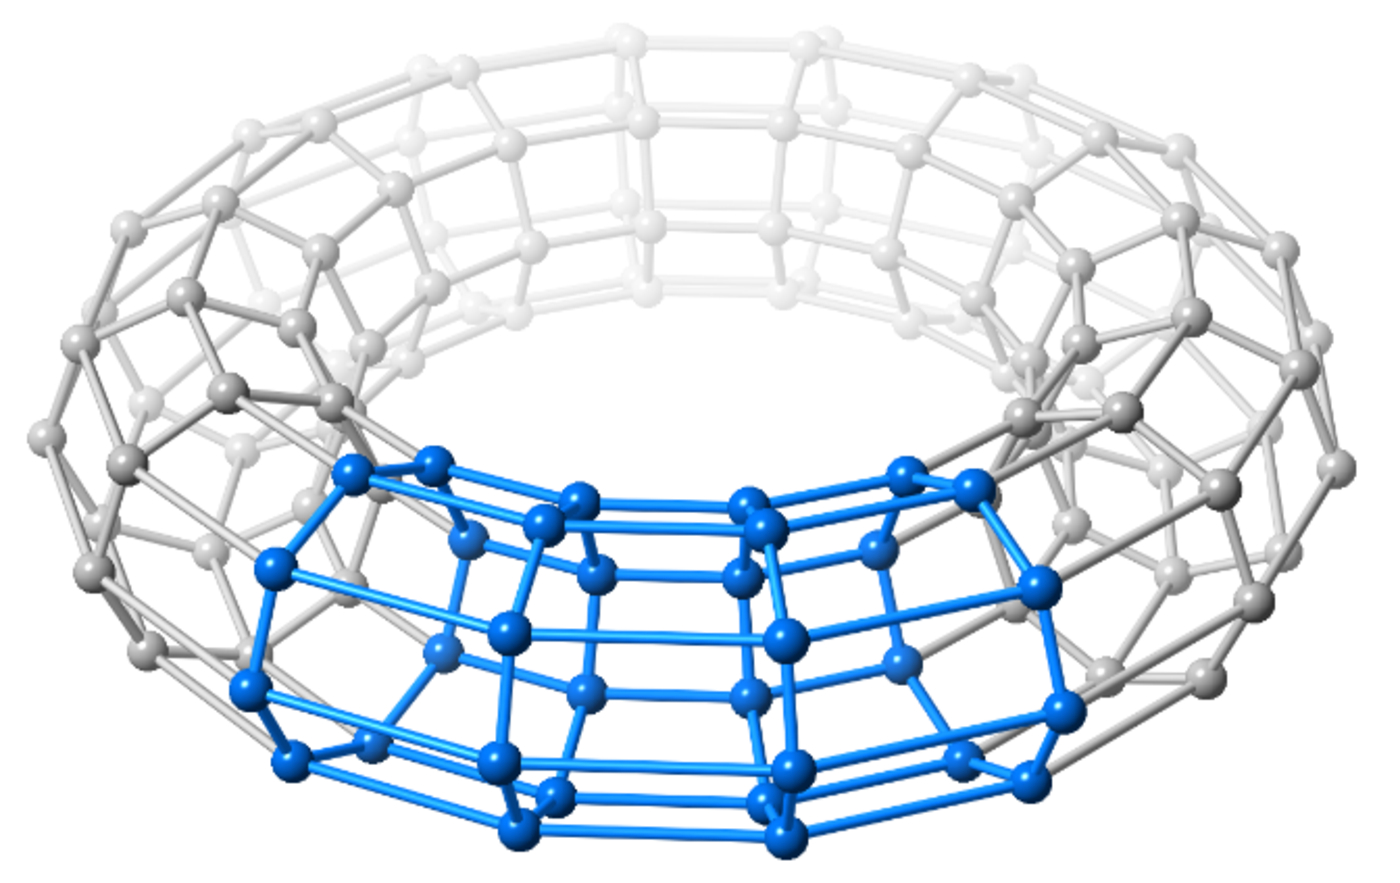
\includegraphics[]{./figs/16x8b.pdf}}
	\end{center}
	\caption{A $8\times16$ torus. Compute entanglement entropy using the SWAP operator and the ratio trick}
	\label{fig:torus}
\end{figure}
%

\section{Entropy scaling of the SU(N) wavefunction}

%
\begin{figure}[h]
	\begin{center}
	\scalebox{0.35}{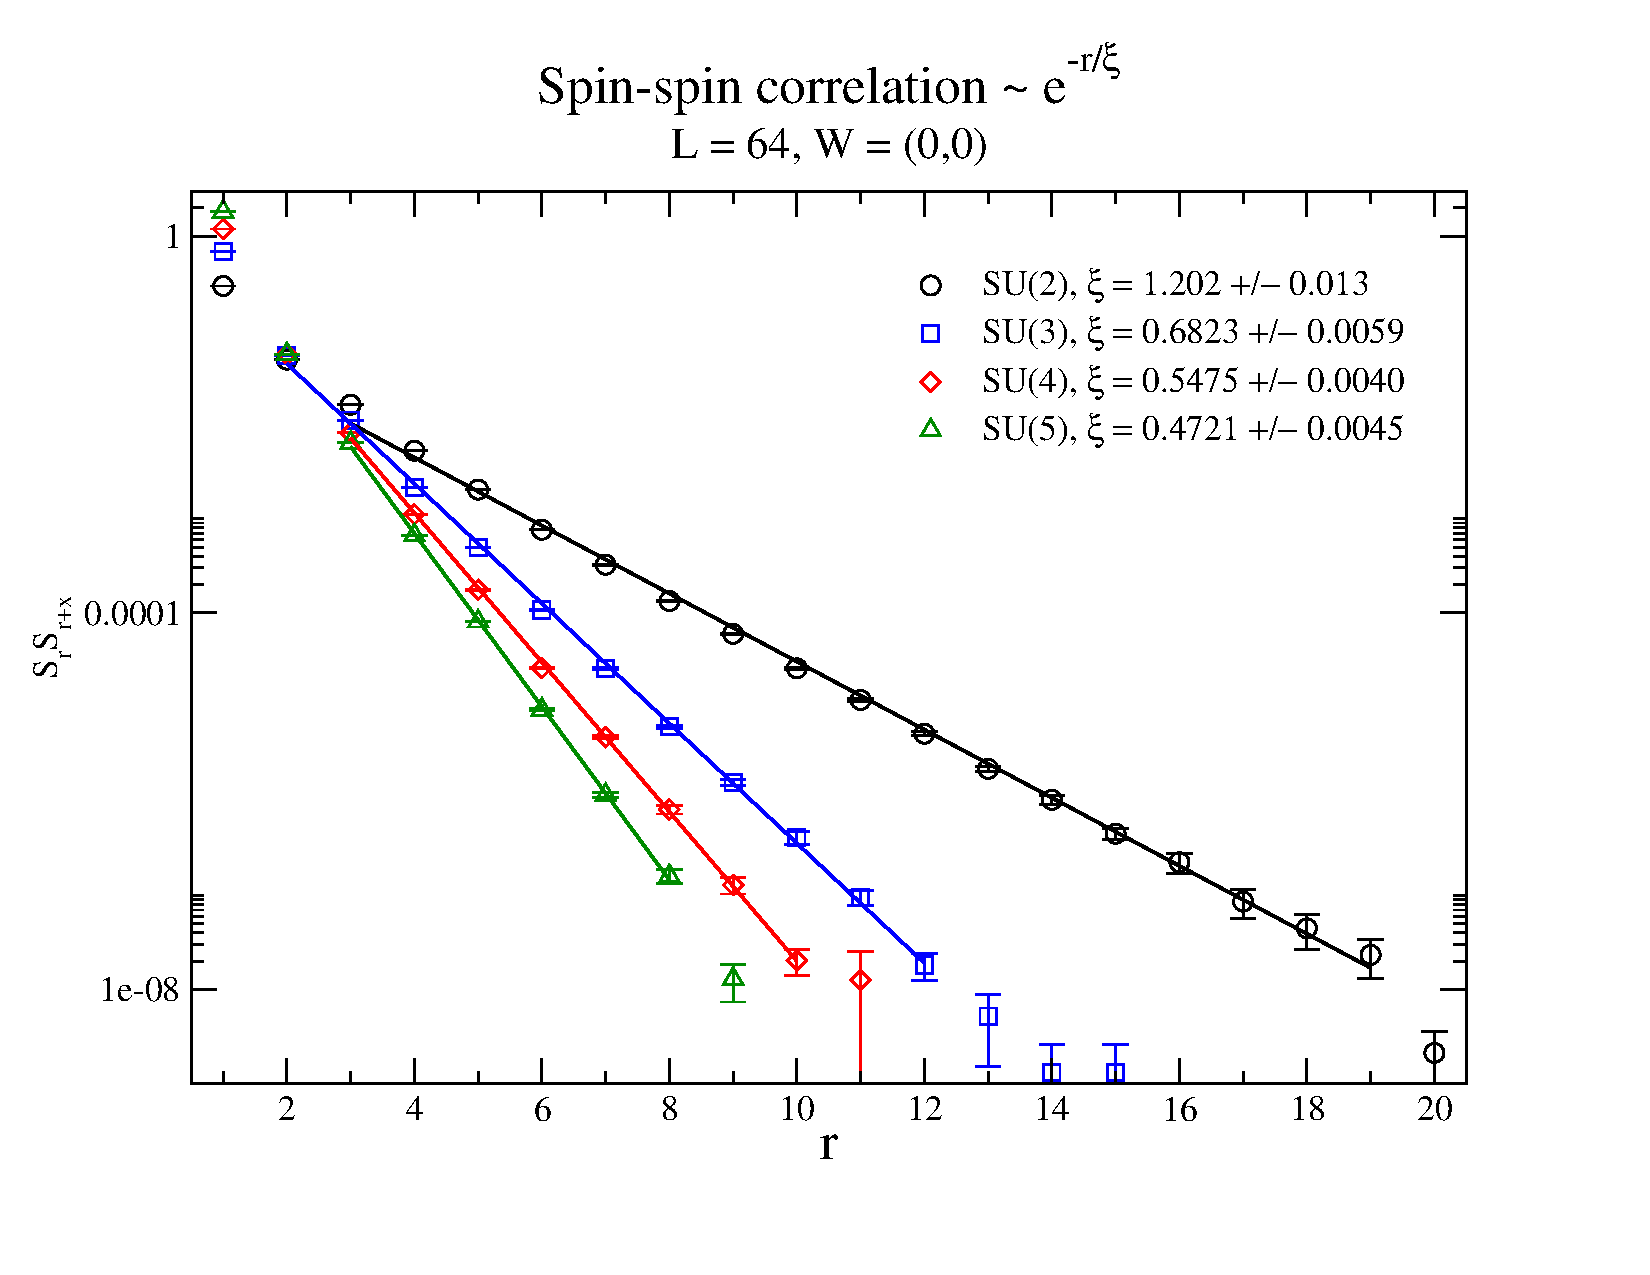
\includegraphics[]{./figs/64-spin.pdf}}
	\end{center}
	\caption{Spin-spin correlations are exponentially decaying and the correlation length is inversely proportional to $N$.}
	\label{fig:dimer64}
\end{figure}
%
%
\begin{figure}[h]
	\begin{center}
	\scalebox{0.35}{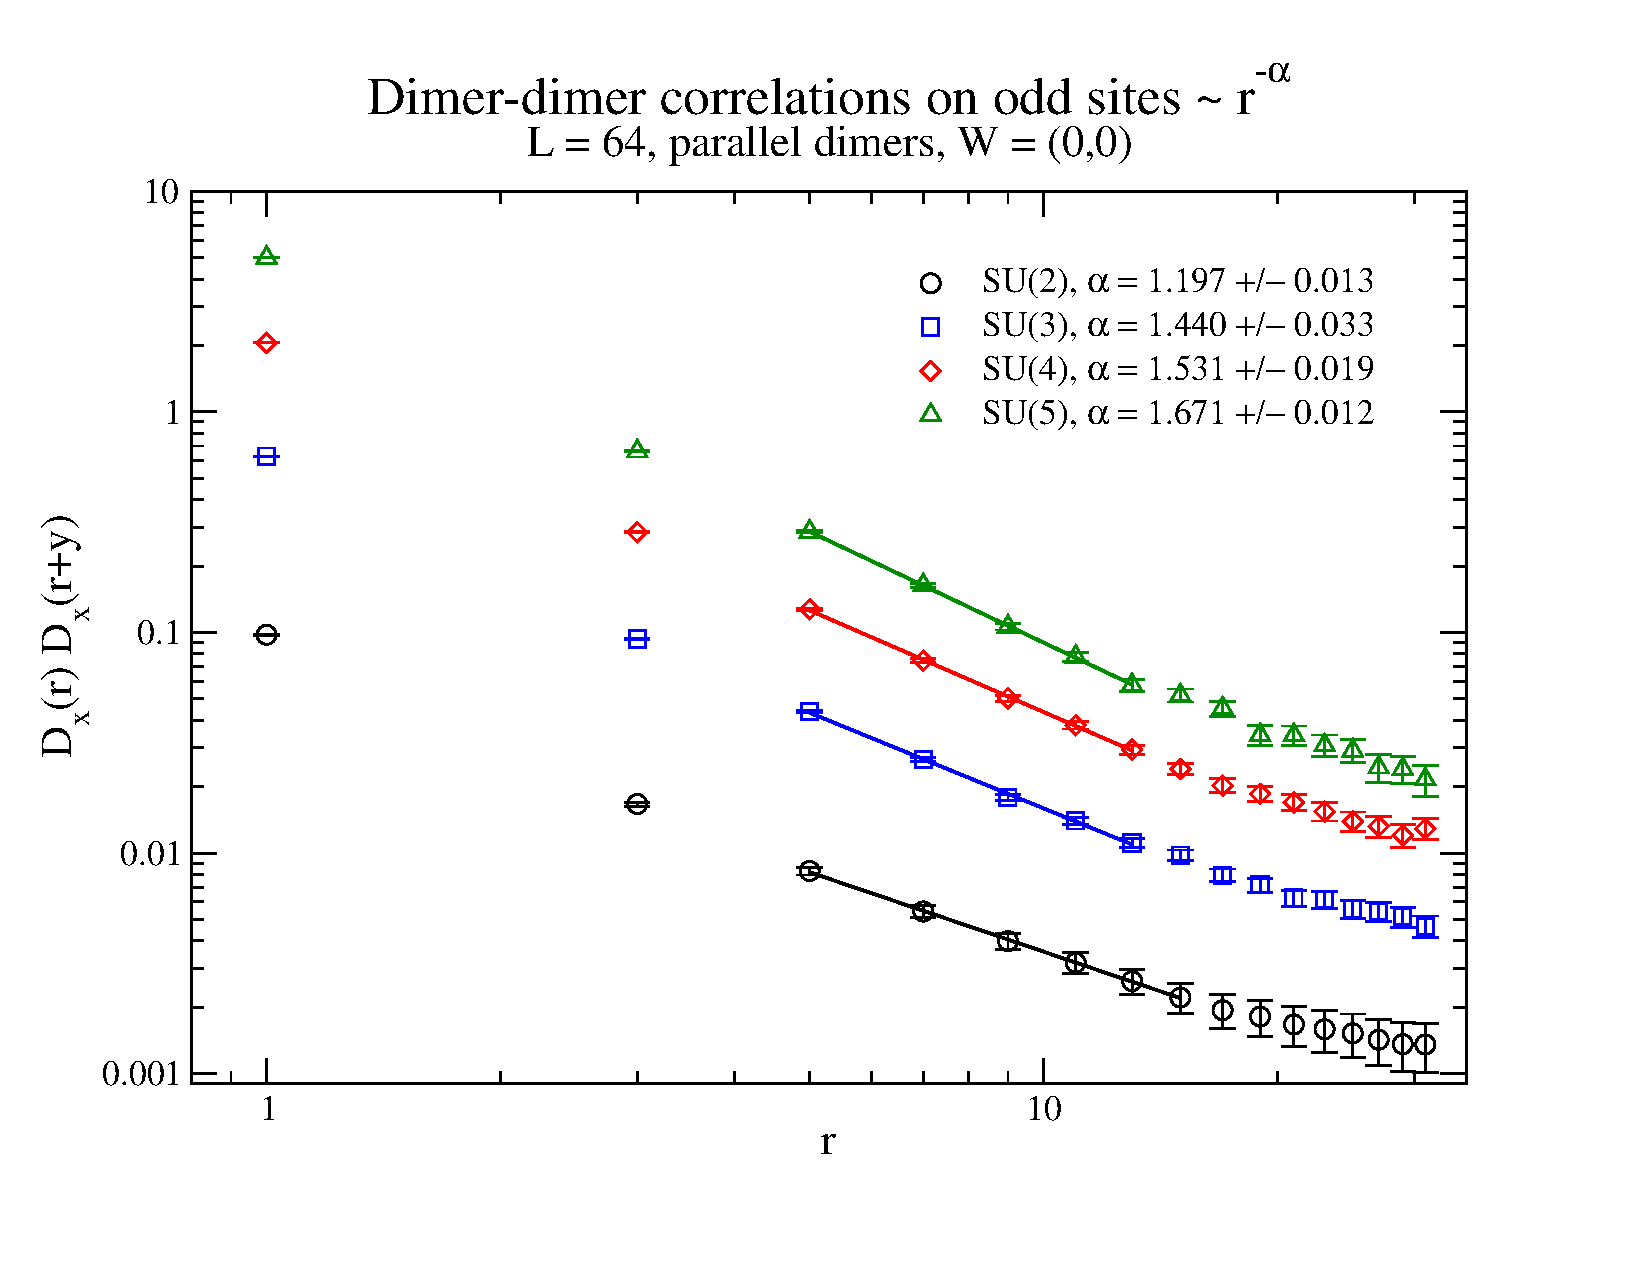
\includegraphics[]{./figs/64-odd-dimer.pdf}}
	\end{center}
	\caption{Critical dimer-dimer correlations for all $N$. We know that the classical value, $N \to \infty$, is $\alpha = 2$. This seems to be saying that SU(3) is not 
			close to being classical.}
	\label{fig:dimer64}
\end{figure}
%
%
\begin{figure}[h]
	\begin{center}
	\scalebox{0.35}{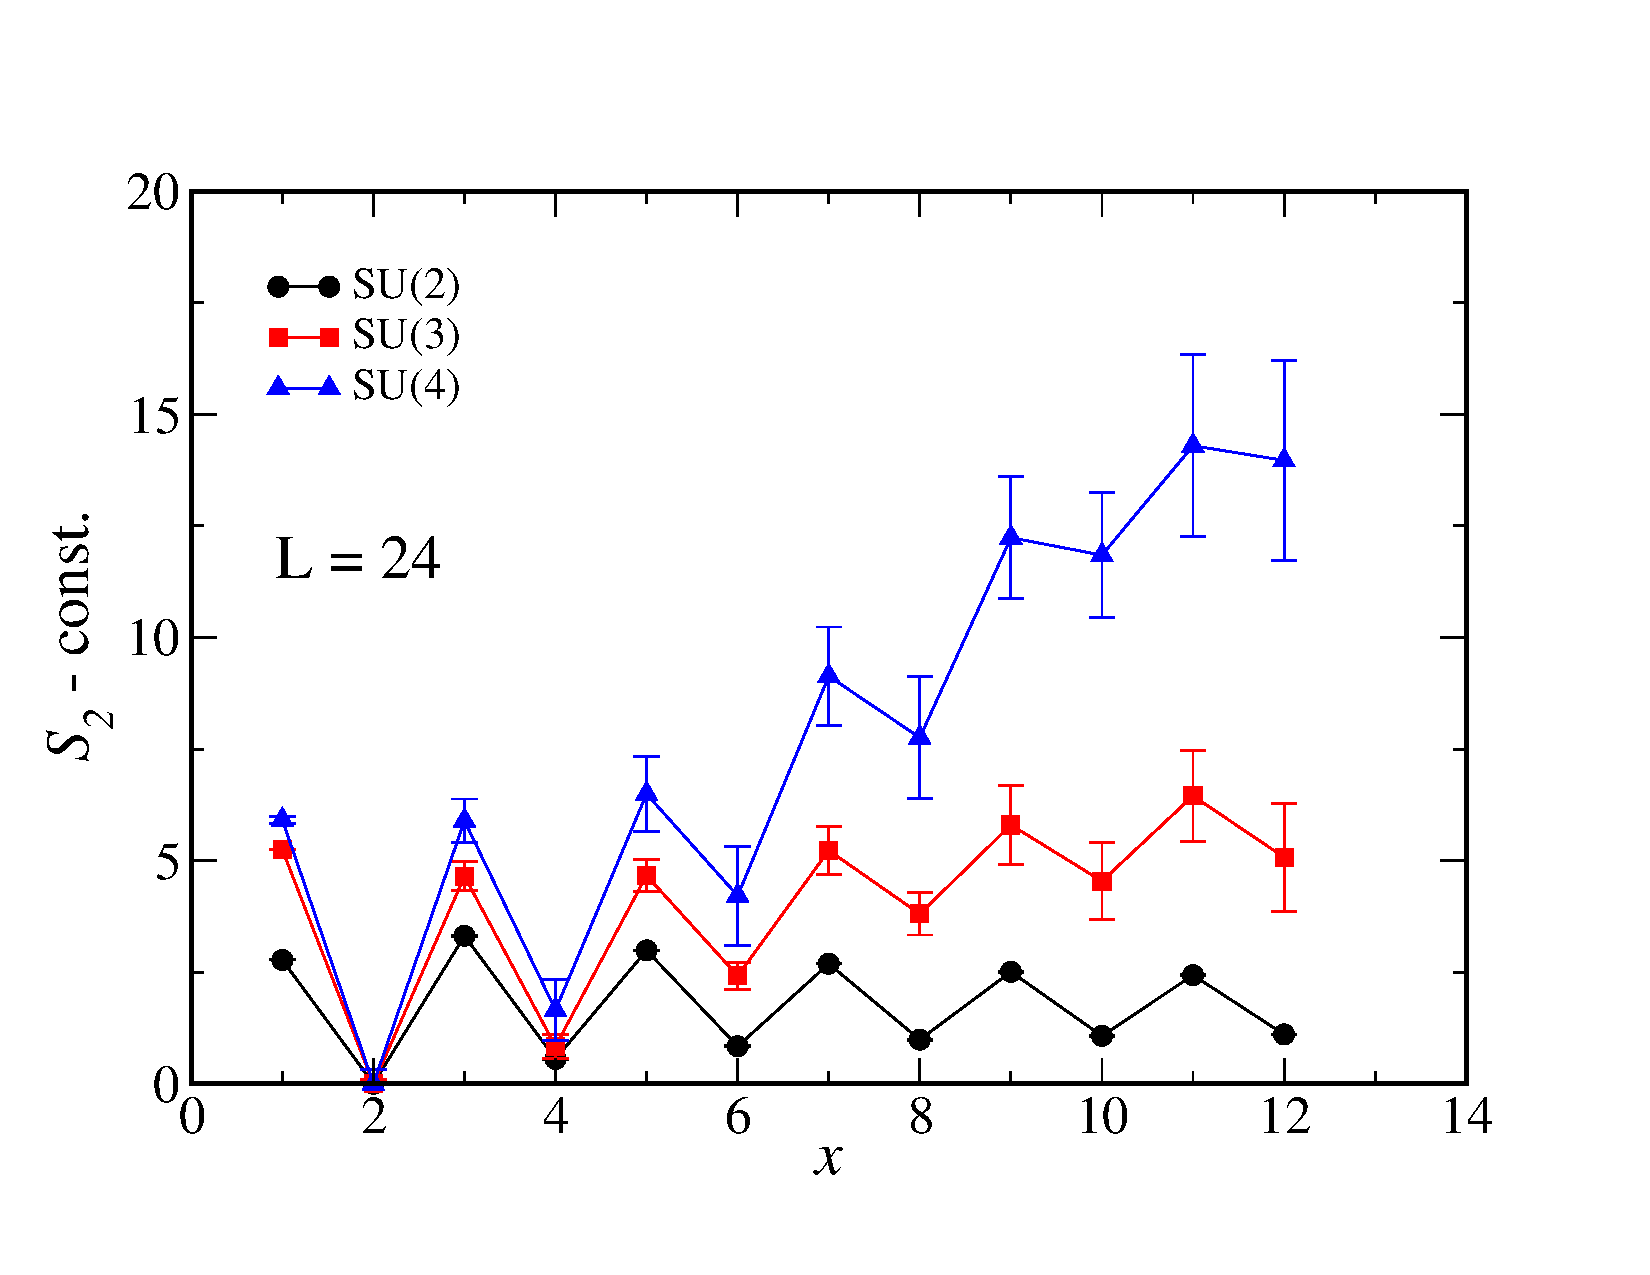
\includegraphics[]{./figs/L24-sun.pdf}}
	\end{center}
	\caption{Prelim figure. Shows the behavior of the entanglement entropy as a function of N. Still trying to converge the SU(3) and SU(4) data. This alone is probably
			not enough to give any conclusive statements about larger $N$, but maybe we can use the dimer-dimer correlations.}
	\label{fig:L24}
\end{figure}
%

%
\begin{figure}[h]
	\begin{center}
	\scalebox{0.35}{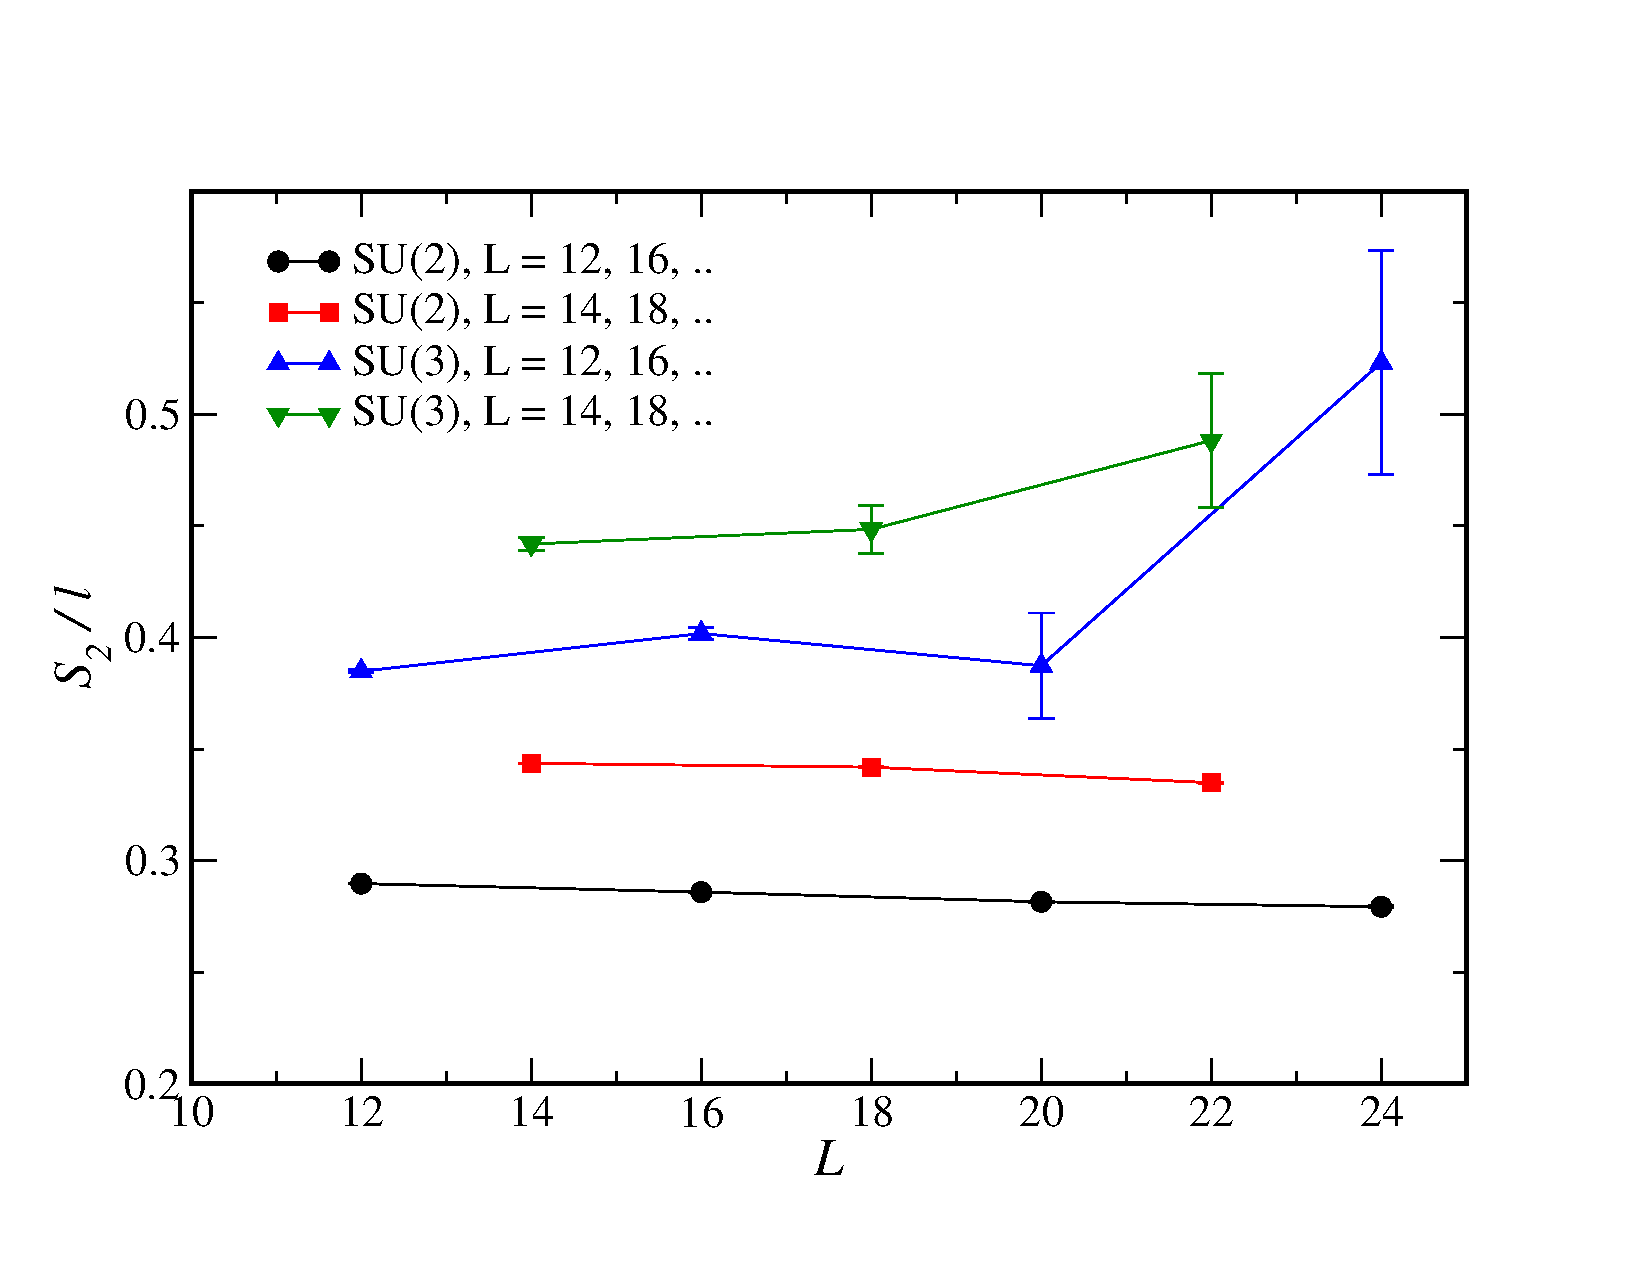
\includegraphics[]{./figs/half-width.pdf}}
	\end{center}
	\caption{Entanglement entropy taken at $x = L/2$ for those that end on even/odd branch. This is probably not necessary. One thing that might be helpful though is to 
			fit the SU(3 or 4) data to $\ln\left[ \sin( \pi x/L ) \right]$ and fit its coefficient.}
	\label{fig:halfwidth}
\end{figure}
%

\section{Jean-Marie's calculations?}

\end{document}